\usepackage{titling}

\renewcommand{\maketitle}{

  \begin{titlepage}
    \begin{center}

      
\includegraphics[width=\textwidth]{./upatras-header.png}

      \vspace*{1.4cm}
      \Large\textbf{ΕΞΑΓΩΓΗ ΣΧΕΣΙΑΚΩΝ ΠΛΗΡΟΦΟΡΙΩΝ ΑΠΌ ΤΗ ΒΙΚΙΠAIΔΙΑ}

      \vspace{2.8cm}
      ΔΙΠΛΩΜΑΤΙΚΗ ΕΡΓΑΣΙΑ

      \vspace{0.8cm}
      \large{\theauthor}


      \vfill

      %% A thesis submitted in partial fulfillment\\
      %% of the requirements for graduation from the\\
      %% Department of Physics


      \vspace{2.2cm}
      ΕΠΙΒΛΕΠΟΝΤΕΣ: Κυριάκος Σγάρμπας, Boris Katz

      \vspace{0.6cm}
      \large
      ΠΑΤΡΑ --- ΜΑΙΟΣ 2016
    \end{center}
  \end{titlepage}
  \clearpage

  \begin {center}

  \def\vs{1.1cm}
  \Large\textbf{ΠΙΣΤΟΠΟΙΗΣΗ}

  \vspace{\vs}
  {Πιστοποιείται οτι η διπλωματική εργασία με θέμα}

  \vspace{\vs}
  \Large\textbf{\thetitle}

  \vspace{\vs}
  {Του φοιτητή του τμήματος Ηλεκτρολόγων Μηχανικών & Τεχνολογίας Υπολογιστών}

  \vspace{\vs}
  \large\textbf{\theauthor}

  \large\textbf{(A.M. 7361)}

  \vspace{\vs}

{Παρουσιάστηκε δημόσια και εξετάστηκε στο Τμήμα
  Ηλεκτρολόγων Μηχανικών & Τεχνολογίας Υπολογιστών στις 8/6/2016}

  \vspace{\vs}
  \vspace{\vs}
  \begin{minipage}{0.45\textwidth}
        \begin{center}
                Ο επιβλέπων

                \vspace{\vs}
                \textbf{Κ. Σγαρμπας}

                \textbf{Επ. Καθηγητής}
        \end{center}
  \end{minipage}%
  \begin{minipage}{0.45\textwidth}
        \begin{center}
                Ο Διευθυντής του Τομέα

                \vspace{\vs}
                \textbf{Ν. Φακωτάκης}

                \textbf{Καθηγητής}
        \end{center}
  \end{minipage}%

  \end {center}

  \clearpage

\large\textbf{Τίτλος:}

\thetitle

    \begin{minipage}{.8\textwidth}
    \large\textbf{Συγγραφέας}

    \theauthor

    (A.M. 7361)
    \end{minipage}
    \begin{minipage}{.2\textwidth}
    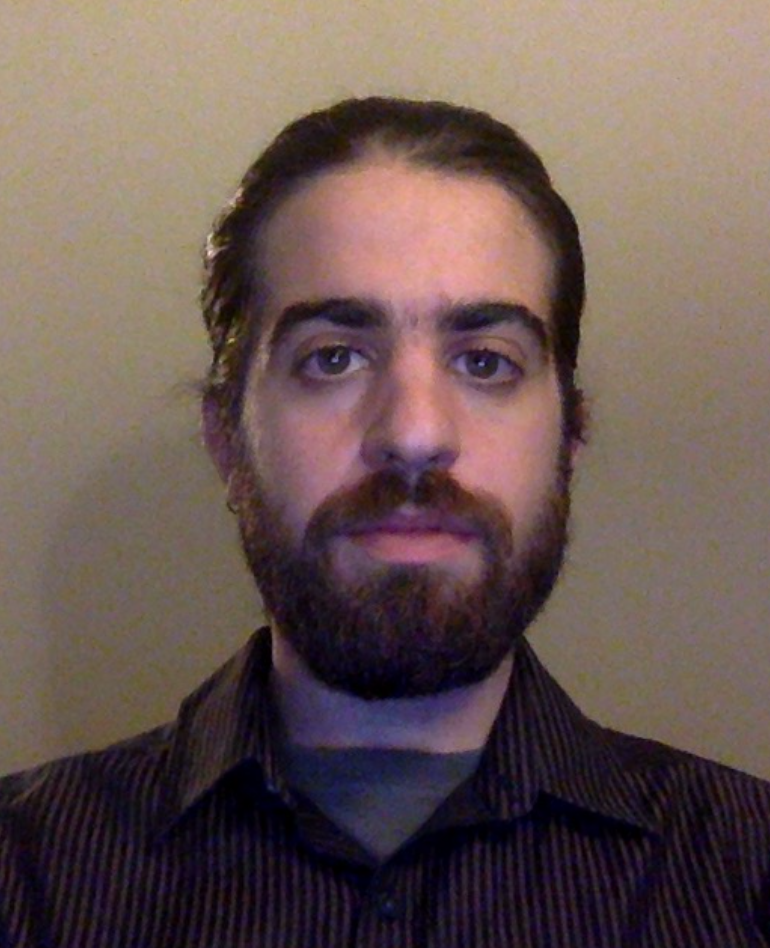
\includegraphics[width=\linewidth]{me.png}
    \end{minipage}

\large\textbf{Περίληψη}

  Το START (SynTactic Analysis using Reversible Transformations) είναι
  ένα πακέτο λογισμικού γραμμένο σε γλώσσα Common Lisp το οποίο αντλεί
  πληροφορίες από διαδικτυακές πηγές και τις χρησιμοποιεί για
  απαντήσει σε αυθαίρετες ερωτήσεις που δέχεται. Αναπτύχθηκε στο
  εργαστήριο Infolab του MIT. Για τον εμπλουτισμό των πληροφοριών που
  χρησιμοποιεί το START χρησιμοποιείται το πακέτο λογισμικού Omnibase
  μέσω του οποίου επιτυγχάνεται πρόσβαση του START σε πολλαπλές πήγες
  στο διαδίκτυο. Στην παρούσα εργασία αναπτύσσουμε μια επέκταση του
  Omnibase που επιτρέπει την πρόσβαση του START στην wikipedia και
  στις πληροφορίες που αυτή περιέχει. Η επέκταση αυτή του Omnibase
  ονομάζεται wikipediabase.  Για την ευκολότερη πρόσβαση του START στη
  Wikipedia δημιουργήσαμε ένα πρόγραμμα (wikipedia-mirror) που
  δημιουργεί κλώνους της Wikipedia που αποθηκεύονται τοπικά ανεξάρτητα
  από το διαδίκτυο.  Έτσι επιτυγχάνεται ταχύτερη και πιο αξιόπιστη
  πρόσβαση του START στο σύνολο των δεδομένων της wikipedia.

\vfill

\large\textbf{Abstract}

  START (SynTactic Analysis using Reversible Transformations) is a
  piece of sofware written in common lisp that retrieves information
  from internet resources and uses them to answer to arbitrary natural
  language questions. It was developed in InfoLab of MiT. For the
  enrichment of the retrieved information it uses the Omnibase
  software through which START gets access to multiple sources on the
  internet. In the present thesis we present an extension to Omnibase
  that allows START to get access to wikipedia and the information
  that it contains. This extension to Omnibase is called
  WikipediaBase. For easier access to wikipedia we also developed a
  separate program (wikipedia-mirror) that creates clones of wikipedia
  running locally and independently to the internet. This way faster
  and more reliable access to wikipedia is accomplished.


\clearpage

  \thispagestyle{plain}
  \vspace*{1in}
  \begin{center}
    \begin{Large}
      \textit{Ευχαριστίες}
    \end{Large}
  \end{center}

  Πρώτα απ όλα θα ήθελα να ευχαριστήσω τους επιβλέποντες μου κ. Κυριάκο
  Σγάρμπα και Dr Boris Katz. Χωρίς την ανεκτίμητη βοήθεια τους η εργασία
  αυτή δε θα γινόταν πραγματικότητα.

  Αδράττω αυτή την ευκαιρία για να εκφράσω τις ευχαριστίες μου σε όλα τα
  μέλη της Ακαδημαϊκής κοινότητας του Τμήματος Ηλεκτρολόγων Μηχανικών
  και Τεχνολογίας Υπολογιστών του Πανεπιστημίου Πατρών και του MiT
  InfoLab για την υποστήριξή τους καθ όλη τη διάρκεια των σπουδών μου.


  Τέλος ευχαριστώ τους γονείς μου και όλους όσους με στήριξαν σε αυτή
  μου την προσπάθεια.

  \afterpage{\blankpage}
  \newpage

  \thispagestyle{plain}
  \vspace*{1in}
  \begin{center}
    \begin{Large}
      \textit{Πρόλογος}
    \end{Large}
  \end{center}

  Το τεχνικό μέρος αυτής της εργασίας (development) εκπονήθηκε κατά το
  έτος 2014-2015 στο MiT InfoLab CSAIL υπό την επίβλεψη των Dr
  Κυριάκου Σγάρμπα του Πανεπιστημίου Πατρών και dr Boris Katz του MiT
  CSAIL. Η συγγραφή του κειμένου πραγματοποιήθηκε στις αρχές του έτους
  2016. Το WikipediaBase ενσωματώθηκε στο δίκτυο του CSAIL προκειμένου
  να χρησιμοποιηθεί από το START στα μέσα του έτους 2015.

  \afterpage{\blankpage}


}
